\documentclass[11pt]{article}
\usepackage[utf8]{inputenc}
\usepackage[T1]{fontenc}
\usepackage[a4paper]{geometry}
\usepackage{comment}
\usepackage{minted}
\usepackage{multirow}
\usepackage{enumerate}
\usepackage{tikz}
\usepackage{enumitem}
\usepackage{fancyhdr}

% pagestyle{fancy} switches on additional headers and footers of the
% fancyhdr package.
%\pagestyle{fancy}
\lhead{BI229F 16.06.2017}
\rhead{\thepage /12}
\renewcommand{\headrulewidth}{0.4pt}
%% for listings..
\definecolor{mintedBg}{rgb}{0.95, 0.95, 0.95}
\definecolor{blockBg}{rgb}{0.6, 0.6, 0.95}
\newminted{perl}{linenos, bgcolor=mintedBg, fontsize=\footnotesize}
\newminted{r}{linenos, bgcolor=mintedBg, fontsize=\footnotesize}
\newminted{console}{linenos, bgcolor=mintedBg, fontsize=\footnotesize}

\specialcomment{Notes}{%
  \begingroup\small\color{red}}{%
  \endgroup}
\excludecomment{Notes}

\setcounter{page}{2}

\begin{document}

This exam contains a total of 8 sections. The majority of these sections have
some choice in the questions that you answer. Please read the instructions
below each section heading. A total of 100 marks will be considered as full marks.

The number of marks available from each section is indicated in the section
headings. Note that it is possible to select questions that total more than
that mark; however, you will not be able to get more marks from a given
section by answering more questions. If you find that your answer to a given
question is no good and you wish to change your selection, then cross out the
old one to indicate which one you do not wish to be marked for.

Feel free to illustrate your answers wherever you feel appropriate; but do
remember to include labels so that I can decipher your figures. Do not include
a picture without some descriptive text. Two of the questions will need to be
filled in on a supplementary sheet. Do not forget to hand this in with your
other answers.

Marks have been assigned on the assumption of a four hour exam; that is one mark
corresponds to 2.4 minutes. For some of the questions that may mean mostly
writing, but for others (esp. code and manual snippets) that time may be taken up by
reading the details of the question, and the answer itself may be very
short.


\section{Bioinformatics in general (12 points)}
Answer questions giving a total of 12 points for this section.
\begin{enumerate}
\item Describe an example where you would need to use a bioinformatics
  analysis. Include both a description of the problem you are concerned with
  and an outline of the analysis you would perform. About half of your answer
  should describe the problem your example is concerned with; the other half
  should describe the approach to solving the problem. Do not go into too much
  detail!\\
  (6 points)\\
\begin{Notes}
  This is an open ended question with no specific answers. I do not expect a
  great deal of detail (eg. specific versions of programs used), but the
  student can receive marks for reasonable answers even if these are not
  technically correct.
\end{Notes}

\item Sequencing:
  \begin{itemize}
    \item How does sequence data differ from (most) other types of data obtained
      in biological research?\\
      (2 points)\\
\begin{Notes}
  Sequence data is qualitative; most other data types are quantitative. This
  makes it easier to define identities. \\
  Students can also get points for other
  reasonable answers, such as the relative cost of obtaining sequence data,
  information density and other such esoteric issues.
\end{Notes}
    \item Describe how sequencing technology has progressed from standard
      Sanger sequencing to the latest next-generation sequencing.\\
      (4 points)\\
\begin{Notes}
  From few long sequences to large numbers of very short (30-50) sequences, to
  very large numbers of intermediate length sequencing (300-600) to the
  latest single molecule based methods giving extremely long (50,000)
  reads. Points for giving names of technologies, their capacities and
  lengths, but I do not expect all technologies or exact numbers to be
  recalled; the most important point is to give the relative trend in
  terms of capacity and read length.
\end{Notes}
  \end{itemize}
\item In the literature you will frequently see the terms 'genomics' and
  'transcriptomics'. What is meant by these terms? Give two examples of the type
  of questions addressed by both.\\
  (6 points)\\
\begin{Notes}
  Genomics and transcriptomics: the study of complete genomes and or
  transcriptomes; i.e. the study of the full set of DNA sequences (genomes) or
  RNA sequences (transcriptome) present in an organism (genome) or cell type
  (transcriptome). Questions may address the properties of the full set of
  data, eg. distribution of genes and repetitive sequences across the genome,
  and or the distribution of gene expression levels. However, the terms are
  most frequently used to describe data mining operations where the activity
  or influence of small number of individual gene or gene features are
  identified from the full 'ome. The student may give any reasonable example
  of question addressed (eg. changes in gene expression induced by external
  factors, identification of mutations associated with a phenotype, comparison
  of whole genomes to infer evolutionary history, etc.).
\end{Notes}
\end{enumerate}

\section{Molecular Biology \& the Central Dogma (20 points)}
Answer questions giving a total of 20 points for this section.
\begin{enumerate}
\item Describe how proteins are encoded in genomes and how this code is read
  to synthesize specific proteins. Include a description of
  how this differs in eukaryotes and prokaryotes as well as details about the
  encoding of amino acids.\\
  (10 points)
\begin{Notes}
  Encoding of amino acid in triplet code; allows encoding of 64 identities,
  but only 20 amino acids; hence redundant. Doublet code too short for 20
  amino acids. Eukaryotes, code for single protein split across several exons
  seperated by introns in a single transcription unit. Prokaryotes, code for
  several proteins contained in a single multicistronic message.
  Transcription to RNA, export (in eukaryotes), translation at ribosomes
  through the assembly of tRNA.
\end{Notes}

\item Given a genetic code:\\
  \begin{minipage}{0.6\textwidth}
  {\tiny
    %% this requires 
%% usepackage{multirow}
%% usepackage{tabularx}

\renewcommand{\arraystretch}{1.25}
\begin{tabular}{ |l| l l|l l| l l|l l|l| }
  \hline
  \multirow{2}{2em}{1st base} &
  \multicolumn{8}{|c|}{2nd base} &
  \multirow{2}{2em}{3rd base} \\
  \cline{2-9}
  &
  \multicolumn{2}{|c|}{U} &
  \multicolumn{2}{|c|}{C} &
  \multicolumn{2}{|c|}{A} &
  \multicolumn{2}{|c|}{G} & \\
  \hline
  \multirow{4}{2em}{U} & 
  UUU & \multirow{2}{4em}{\tiny (Phe/F)} &
  UCU & \multirow{4}{4em}{\tiny (Ser/S)} &
  UAU & \multirow{2}{4em}{\tiny (Tyr/Y)} &
  UGU & \multirow{2}{4em}{\tiny (Cys/C)} & U \\
  & UUC & & UCC & & UAC & & UGC & & C \\ \cline{2-3} \cline{6-9}
  & UUA & \multirow{6}{4em}{\tiny (Leu/L)} 
  & UCA & & UUA & Stop & UGA & (Stop) & A \\ \cline{8-9}
  & UUG & & UCG & & UAG & Stop & UGG & \tiny (Trp/W) & G \\ \cline{4-9} 
  \cline{1-1}
  \multirow{4}{2em}{C}
  & CUU & & CCU & \multirow{4}{4em}{(Pro/P)} & CAU & \multirow{2}{4em}{(His/H)} & CGU & \multirow{4}{4em}{(Arg/R)} & U \\
  & CUC & & CCC & & CAC & & CGC & & C \\ \cline{6-7}
  & CUA & & CCA & & CAA & \multirow{2}{4em}{Gln/Q} & CGA & & A \\
  & CUG & & CCG & & CAG & & CGG & & G \\ \cline{1-9}
  \multirow{4}{2em}{A}
  & AUU & \multirow{3}{4em}{(Ile/I)} & ACU & \multirow{4}{4em}{(Thr/T)} & AAU 
  & \multirow{2}{4em}{(Asn/N)} & AGU & \multirow{2}{4em}{(Ser/S)} & U \\
  & AUC & & ACC & & AAC & & AGC & & C \\ \cline{6-9}
  & AUA & & ACA & & AAA & \multirow{2}{4em}{(Lys/K)} & AGA & \multirow{2}{4em}{(Arg/R)} & A \\
  \cline{2-3}
  & AUG & (Met/M) & ACG & & AAG & & AGG & & G \\ \cline{1-9}
  \multirow{4}{4em}{G}
  & GUU & \multirow{4}{4em}{(Val/V)} & GCU & \multirow{4}{4em}{(Ala/A)} 
  & GAU & \multirow{2}{4em}{(Asp/D)} & GGU & \multirow{4}{4em}{(Gly/G)} & U \\
  & GUC & & GCC & & GAC & & GGC & & C \\ \cline{6-7}
  & GUA & & GCA & & GAA & \multirow{2}{4em}{(Glu/E)} & GGA & & A \\
  & GUG & & GCG & & GAG & & GGG & & G \\ \hline
\end{tabular}

  }
  \end{minipage}

  Given the following (double stranded!) genomic sequence:\\
  \verb|5' GCGATGGGCGGTGGGGTG 3'|\\
  determine all possible translations.\\
  (4 points)

\begin{Notes}
  6 translations, 3 forward, 3 reverse, beginning with 'Ala,Met,...'
\end{Notes}

\item What kind of mutations can arise in DNA sequences? Explain how the
  consequences of these mutations differ depending on the type of mutation and
  where in the genome the mutation happens.\\
  (6 points)

\begin{Notes}
  substitutions, insertions / deletions, translocations. Substitutions inside ORFs
  can lead to changes in protein sequence and premature stops, inserts /
  deletions lead to frame shift. Translocations can lead to gene fusions
  and changes in gene expression. Point mutations outside of genes generally
  have no effect.
\end{Notes}

\item How do the monomers of nucleic acids differ from those of proteins? How
  does this relate to their function and to the fact that DNA is usually double-stranded?\\
(6 points)

\begin{Notes}
  The monomers of nucleic acids are structurally similar to each other; this
  means that the sequence of a nucleic acid molecule has little effect on its
  structure. The double-stranded nature of DNA decreases the structural
  influence of the primary sequence. The primary function of nucleotide
  polymers is to encode information; this function would be compromised if the
  sequence also had a strong effect on physical structure. In contrast the
  function of proteins arises from their structure and this is facilitated by
  the variety of chemical structures present in different amino acids.
\end{Notes}
\end{enumerate}

\section{ Biological databases \& formats (8 points) }
Answer questions giving a total of 8 points for this section.
\begin{enumerate}
\item Given an approximatly 1000 base-pair long nucleotide sequence what would
  you do to identify the source and function of the sequence? Give some
  details as to what types of databases you would use.\\
  (8 points)

\begin{Notes}
  Search nucleotide databases for similar or identical sequences; determine if
  sequence is likely to be transcribed and or translated by looking at the the
  sequences it matches. If transcribed, then find function from genome
  databases like ensembl and species functional databases (eg. mouse genome
  informatics / zfin). If no identical sequences found use closest homologue,
  and use orthology to extend functional annotation. If sequence is not
  transcribed, but genomic match is found then find adjacent genes and get
  function of those, to get an idea; also consider looking at extent of
  conservation across species (available from genome databases like
  ensembl).\\
  The above is an example of what can be done. But there are many more
  options and different ways to answer this question.
\end{Notes}

\item Describe the fastq and fasta sequence formats.\\
(4 points)

\begin{Notes}
  Indicate how headers, sequence and quality data are distinguished in these files.
\end{Notes}

\item The SAM format is used to describe the alignments of large numbers of
  sequences to a common reference sequence (typically a genome sequence). Each
  alignment is described by a single line of tab delimited text. The second
  field of this description is a FLAG that uses a single number to encode
  speficic combinations of 12 flags that indicate individual
  properties of problems of the sequences or alignments as indicated by the
  following table:

  {\small
  \begin{tabular}{rrl}
    Bit & Value & Description\\
    \hline
    1 & 1 & template having multiple segments in sequence \\
    2 & 2 & each segment properly aligned according to the aligner\\
    3 & 4 & segment unmapped\\
    4 & 8 & next segment in the template unmapped\\
    5 & 16 & SEQ being reverse complemented\\
    6 & 32 & SEQ of the next segment in the template being reverse complemented\\
    7 & 64 & the first segment in the template\\
    8 & 128 & the last segment in the template\\
    9 & 256 & secondary alignment\\
    10 & 512 & not passing filters, such as platform quality controls\\
    11 & 1024 & PCR or optical duplicate\\
    12 & 2048 & supplementary alignment\\
  \end{tabular}
  }

  Each 'Value' in the above table is an exact power of 2 which means that it
  is encoded in binary by a single 1 in the indicated position. A single
  number can thus hold any combination of the given flags. For example, if a
  given sequence failed to pass filters, and has been reverse complemented we
  set the 10th (512) and 5th (16) bits to 1 giving us 528 (512 +
  16) which is represented in binary as: \verb|001000010000|.\\ 
  Give the binary encodings and describe the meanings of the following 
  FLAG values: 147, 99, 98. Which one of these does not make sense and why?\\ 
  (4 points)

\begin{Notes}
  147 = 128 + 16 + 2 + 1 = 000010010011 $\Rightarrow$ multiple segments,
  each segment properly aligned, sequence reverse complemented, last segment
  in template\\
  99 = 64 + 32 + 2 + 1 = 000001100011 $\Rightarrow$ multiple segments,
  each segment properly aligned, sequence of next segment reverse
  complemented, first segment in the template\\
  98 as 99, but flag for multiple segments not set; hence does not make
  sense as the flags refer to other segments in the template.
\end{Notes}

\end{enumerate}

\section{Pairwise alignment (20 points)}
Answer questions giving a total of 20 points for this section.
\begin{enumerate}
\item Given the two sequences \verb|5' GCTATGA 3'| and \verb|5' GTTTA 3'|\\
  \begin{itemize}
    \item Provide at least two reasonable alignments
    \item Describe how you can score the alignments using a set of penalties
      or scores.
    \item Score the alignments using your own scoring system. Which of your
      alignments is the best and how does this relate to your scoring system?
    \item Are your alignments global or local? Describe how this affects the
      score.
    \item Describe what is meant by an 'affine gap penalty'. Does it have any
      effect on your alignments?
  \end{itemize}
  (10 points)

\begin{Notes}
  Any reasonable alignment is OK. These should be scored by match scores, 
  and penalties for mismatches and gap insertions. Generally the hightest
  scoring alignment is the best; but changing the scoring system can change
  which has the highest score. The alignments are global if gap penalties
  have been included for terminal gaps; otherwise local. Global gives lower
  scores. Affine gap penalty: different penalties for gap insertion and gap
  extension. In this case unlikely to have any effect as no reasonable way
  to insert a double gap (as far as I can see anyway).
\end{Notes}

\item Fill in the first three rows and columns of the following alignment
  table for a global alignment (Needleman-Wunsch). Include both scores and
  back-track information (Use the supplementary sheet).
  \begin{figure}[H]
    \begin{tikzpicture}[scale=0.6]
      \input{2016_june_tikz/needleman_1_b.tikz}
    \end{tikzpicture}
  \end{figure}
  (6 points)

\begin{Notes}
  Although there is a single correct answer here, the student can gain marks
  by partial completion or demonstration of a partial understanding;
  eg. following rules for Smith Waterman, or getting everything right except
  the rules of affine gap penalties.
  
  First three rows and columns of:\\
  \begin{figure}[H]
    \begin{tikzpicture}[scale=0.6]
      \input{2016_june_tikz/needleman_1_a.tikz}
    \end{tikzpicture}
  \end{figure}
\end{Notes}

\item What does the following figure contain? Obtain all optimal alignments
  from it:
  \begin{figure}[H]
    \begin{tikzpicture}[scale=0.6]
      \input{2016_june_tikz/smith_water_1_b.tikz}
    \end{tikzpicture}
  \end{figure}
  \begin{enumerate}
  \item Draw the process directly on the table on the supplementary sheet.
  \item Write the alignments you obtained from it in the main answer sheet.
  \item What kind of alignment(s) did you obtain?
  \end{enumerate}
  (6 points)

\begin{Notes}
  \begin{figure}[H]
    \begin{tikzpicture}[scale=0.6]
      \input{2016_june_tikz/smith_water_1_a.tikz}
    \end{tikzpicture}
  \end{figure}
\end{Notes}

\item Amino Acid substitution matrices:
  \begin{enumerate}
  \item What are substitution matrices and how do we use them when aligning
    sequences?\\
    (2 points)
\begin{Notes}
  tables that provide mismatch penalties for amino-acid pairs. They are used
  instead of a single mismatch penalty, such that more dissimilar amino acids
  give higher penalties.
\end{Notes}
  \item Describe at least two ways in which you can derive an amino acid
    substitution matrix?\\
    (4 points)
\begin{Notes}
  examples include: mutation distances, physical similarities and based on the
  frequencies observed in alignments of homologous sequences.
\end{Notes}
%%   \item On what basis could you define a nucleotide substitution matrix for
%%     aligning DNA sequences?\\
%%     (2 points)
%% \begin{Notes}
%%   different scores for transitions or transversions; or use similar approach
%%   to amino acid sequences using alignments of closely related homologous sequences
%% \end{Notes}
  \item The following is an example of an amino acid substitution table.
    \begin{figure}[H]
      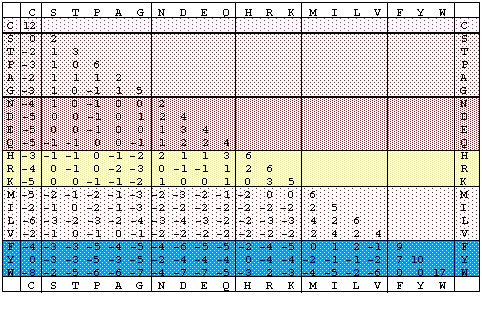
\includegraphics[width=0.7\textwidth]{images/dayhoff_256}
    \end{figure}
    What do the numbers in the matrix indicate?\\
    (4 points)
\begin{Notes}
  Simplest answer is: the penalty added to the alignment score when extending an alignment
  containing the indicated pairs of amino acids. Better answers may refer to
  the frequency of observing the given amino-acid pairs in homologous sequences.
\end{Notes}
  \end{enumerate}
  (10 points)
\item Why do we often use a different penalty for gap insertion and gap
  extension?\\
  (4 points)

\begin{Notes}
  A single event can give rise to a multi-base insertion or deletion; the gap
  extension penalty relates to the relationship between length of the indel
  and the likelihood of it arising. From a functional perspective, lowering
  the penalty for gap extension serves to keep functional units aligned
  (eg. codons, or individual regulatory motifs).  
\end{Notes}
\end{enumerate}

\section{Multiple sequence alignment (10 points)}
Answer questions giving a total of 10 points for this section.

\begin{enumerate}
\item There are two distinct types of homologous sequences. What are they
  called and how do they arise during evolution?\\ 
  (4 points)

\begin{Notes}
  Sequences (or entities) with a common evolutionary origin: orthologues
  across species, paralogues within species, homologues either. Orthologues
  arise as an effect of speciation, paralogues as a result of gene
  duplication.
\end{Notes}

\item Why is it useful to align multiple sequences to each other? Give several
  examples where a multiple sequence alignments are used.\\
  (4 points)

\begin{Notes}
  many potential uses: diagnostic patterns, detection / demonstration of
  homology, prediction of secondary / tertiary structure in proteins,
  suggestion of primer sequences, prelude to phylogenetic analyses, etc.. 
\end{Notes}

\item What are heuristic methods? Why do we use them instead of dynamic
  programming to perform multiple sequence alignment?\\
  (2 points)

\begin{Notes}
  methods which do not guarantee optimal or correct results; typically require
  less computation than optimal methods; but sometimes there may be no known
  optimal methods. Reasonable methods that are shown to work empirically
  rather than proven to do the right thing.
\end{Notes}

\item The Clustal program makes use of a guide tree to perfrom multiple
  sequence alignment. What does this tree represent and how does Clustal
  create this tree?\\
  (6 points)

\begin{Notes}
  the tree represents a model of the evolutionary relationships between the
  individual sequences; branch lengths relate to evolutionary distance and
  tree topology to a hypothesis of the process. The tree is created simply
  from pairwise dis-similarities (a measure of difference between sequences)
  of the sequences aligned to each other (based on the alignment
  scores). These dis-similarities are then used in a neighbour-joining process
  to create the tree through the serial joining of nodes.
\end{Notes}

\item The following figure shows a theoretical guide tree obtained by a
  Clustal analysis. This is used to progressively align sequences and
  alignments to each other. Describe the sequence of alignments carried out by
  Clustal to obtain the final multiple alignment.
  \begin{figure}[H]
    \begin{tikzpicture}[scale=0.5]
    \input{2016_june_tikz/prog_align.tikz}
    \end{tikzpicture}
  \end{figure}
  (4 points)

\begin{Notes}
  \begin{enumerate}
  \item align AB to CD
  \item align FG to E
  \item align ABCD to EFG
  \end{enumerate}
\end{Notes}

\end{enumerate}

\section{Perl (10 points)}
Answer questions giving a total of 10 points for this section.
\begin{enumerate}
\item In Perl what do the following symbols denote: \verb|$ @ %| ? Give
  examples of how they are used in perl code.\\
(4 points)

\begin{Notes}
  \$ a scalar variable\\
  @ an array of variables\\
  \% a key-value hash or map of variables
\end{Notes}

\item What does the following code do?

  \begin{perlcode}
  #!/usr/bin/perl -w
    
  $a = $ARGV[0];
  $b = $ARGV[1];

  print "$a + $b = ", $a + $b, "\n";
  \end{perlcode}
  Explain what kind of errors you may get running the above code.\\
  (4 points)

\begin{Notes}
  Prints the sum of the two first arguments given to the script invocation,
  but does not check that two arguments are given and does not confirm that
  these can reasonable be added to each other (i.e. are numbers).
\end{Notes}

\item Read the following code carefully:

  \begin{perlcode}
  $a = 12;
  $b = 8;
  $c = 0;
  if($a = $b){
    print "$a is equal to $b\n";
  }else{
    print "$a is not equal to $b\n";
  }
  if($a = $c){
    print "$a is equal to $c\n";
  }else{
    print "$a is not equal to $c\n";
  }
  \end{perlcode}
  What will the code print and why?\\
  (6 points)

\begin{Notes}
  \verb|8 is equal to 8|\\
  \verb|0 is not equal to 0|\\
  because \verb| $a = $b | assigns the value of \verb|$a| to \verb|$b| and
  returns the value used in the assignment which evaluates to \verb|TRUE| in
  the conditional. In the second conditional \verb|$a| is
  assigned to the value of \verb|$c| and this value is returned by the
  assignment. Since this value is 0, it evaluates to \verb|FALSE| and the
  second alternative is printed. (Lots of points available as the second
  point is a bit tricky).
\end{Notes}

\item Write Perl code that takes two arguments and then initiates and prints out a Fibonacci
  series from these two arguments (i.e. each value should be equal to the sum of the
  two preceding values in the series). The length of the extension should be given
  by the third argument to the script. Note that your script can assume that
  all arguments given to the script are numeric, and that you will be judged
  more on the logic of your script than the absolute correctness.\\
  (6 points)

\begin{Notes}
  There are many possible answers; the student can get full marks with faulty
  syntax as long as the logic is correct. One example:

\begin{perlcode}
  #!/usr/bin/perl -w
  ($a1, $a2, $l) = @ARGV;
  print "$a1\t$a2";
  for($i=0; $i < $l; $i++){
    print "\t", $a1 + $a2;
    $tmp = $a2;
    $a2 = $a1 + $a2;
    $a1 = $tmp;
  }
  print "\n";
\end{perlcode}
\end{Notes}

\end{enumerate}

\section{Finding homologous sequences (10 points)}
Answer questions giving a total of 10 points for this section.
\begin{enumerate}
\item How would you identify a local alignment between sequence 1 (\verb|LGALSCTCW|) 
  and 2 (\verb|GSLLCTA|) from the following table:
\begin{figure}[H]
  \begin{minipage}[t]{0.5\textwidth}
  {\small
    \setlength{\tabcolsep}{0.5em}
    \begin{tabular}[t]{l|ll|l}
      AA & S2 & S1 & S1-S2 \\
      \hline
      G & 1 & 2 & 1\\
      S & 2 & 5 & 3\\
      L & 3 & 1,4 & -2,1 \\
      L & 4 & 1,4 & -3,0\\
      C & 5 & 6 & 1\\
      T & 6 & 7 & 1\\
      A & 7 & 3 & -4 \\
    \end{tabular}
  }
\end{minipage} 
\begin{minipage}[t]{0.5\textwidth}
  {\small
  Where, \texttt{AA} gives the amino acid residues in sequence 2 located at
  the positions indicated by column \texttt{S2}. Column \texttt{S1} gives
  the lookup table for sequence one. Column \texttt{S1-S2} gives the
  difference between values in \texttt{S1} and \texttt{s2}.
  }
\end{minipage}
  

\end{figure}
Write out the final alignment and score it using the substitution matrix
given in the pairwise alignment section (show your working!).
{\small Hints: It may help you to plot column \texttt{S1} vs
  \texttt{S2}, though this is not necessary.
}\\
(6 points)

\begin{Notes}
  Find the most common offset in the S1-S2 column, and align the two sequences
  from the first to last occurence of this offset in S2 starting at S2 pos +
  offset\\
\begin{verbatim}
    GALSCT
    |*|*||
    GSLLCT
\end{verbatim}
  score = 5 + 1 + 6 + -3 + 12 + 3 = 24
\end{Notes}
\item Give a brief description of the Blast algorithm, describing how it is
  applied when searching a protein sequence against protein sequence
  database. Make sure to explain what High-scoring Segment Pairs are and how these
  relate to the amino acid substitution matrix.\\
(6 points)

\begin{Notes}
  An index is made of the high-scoring pairs of words that can be aligned
  against the query sequence. A high scoring pair is a pair of words (for
  peptide sequences a word is usually 3 or 4 amino acids, for nucleic acid
  sequences usually 11 bp) whose alignment score is higher than a selected
  minimum score; all possible words that can align against the query word are
  thus included in the index. This index is typically much larger than the sequence
  itself. The database of sequences is then scanned against this index; when
  matches are found they are extended until the score goes below a specified
  fraction of the maximal score obtained in the alignment. Later
  implementations do this latter stage using a dynamic programming
  algorithm.\\
  I do not expect a perfect answer here, but something approaching the above.
\end{Notes}

\item The following is part (very simplified) of the output of \texttt{blastn -help}.\\
  \begin{consolecode}
lmj:[R]> blastn -help 
USAGE                                                                                                                                                 
  blastn [-h] [-help] [-import_search_strategy filename]                                                                                              
    [-db database_name] [-query input_file]                                                                            
    [-out output_file] [-evalue evalue] [-strand strand]
    [-gapopen open_penalty] [-gapextend extend_penalty]                                                                                               
    [-max_hsps int_value] [-num_threads int_value] [-remote]
    [-version]

DESCRIPTION
   Nucleotide-Nucleotide BLAST 2.4.0+

OPTIONAL ARGUMENTS
 -help
   Print USAGE, DESCRIPTION and ARGUMENTS; ignore all other parameters
 -version
   Print version number;  ignore other arguments

 *** Input query options
 -query <File_In>
   Input file name
   Default = `-'
 -strand <String, `both', `minus', `plus'>
   Query strand(s) to search against database/subject
   Default = `both'

 *** General search options
 -task <String, Permissible values: 'blastn' 'blastn-short' 
           'dc-megablast' 'megablast' 'rmblastn' >
   Task to execute
   Default = `megablast'
 -db <String>
   BLAST database name
    * Incompatible with:  subject, subject_loc
 -out <File_Out>
   Output file name
   Default = `-'
 -evalue <Real>
   Expectation value (E) threshold for saving hits 
   Default = `10'
 -gapopen <Integer>
   Cost to open a gap
 -gapextend <Integer>
   Cost to extend a gap
 -penalty <Integer, <=0>
   Penalty for a nucleotide mismatch
 -num_threads <Integer, >=1>
   Number of threads (CPUs) to use in the BLAST search
   Default = `1'
  \end{consolecode}

  \begin{enumerate}
  \item 
    Write a command that that will use blastn to search a database called
    \texttt{genome\_db} for matches to sequences in the file \texttt{q\_seq.fa}.\\
    You may assume that the files containing the database are present in the
    current working directory.
  \item How might you modify this command 
    \begin{itemize}
      \item to make blast only report significant alignments that would not be
        expected by chance?
      \item to penalise gaps more?
      \item to make blast run faster?
    \end{itemize}
  \end{enumerate}
  (6 points)
  
\begin{Notes}
  \begin{enumerate} 
  \item \verb|blastn -query q_seq.fa -db genome_db|\\
  \item \verb|blastn -query q_seq.fa -db genome_db -evalue 0.001|\\
    or any number less than 1\\
  \item \verb|blastn -query q_seq.fa -db genome_db -gapopen 10 -gapextend 3|\\
    but this is tricky as the help page doesn't mention what the default value
    is. The answer is to increase the gap penalty using the \verb|-gapopen|
    and \verb|-gapextend| switches reasonably.
  \item use \verb|-num_threads 10| or some other such value.
  \end{enumerate}
\end{Notes}

\item Write down a lookup table (index) for the following sequence:
\begin{verbatim}
TPATGGANWT
\end{verbatim}
Use the amino acid subsitution table from section 4 to identify 2 high scoring segment pairs
that would be included in a blast lookup table and give their scores.\\
 (4 points)

\begin{Notes}
\begin{verbatim}
    T   1,4,10
    P   2
    A   3,7
    G   5,6
    N   8
    W   9
\end{verbatim}
Many examples, but most obvious would be:
\begin{verbatim}
TPA - TPA   3 + 6 + 2
TPA - TPG   3 + 6 + 1
\end{verbatim}
\end{Notes}
\end{enumerate}

\section{Numbers, big data and R (10 points)}
Answer questions giving a total of 10 points for this section.

\begin{enumerate}
%% \item What is meant by 'the distribution of values' and how can you obtain
%%   this in \texttt{R}?\\
%%   (3 points)

%% \begin{Notes}
%% The frequencies of observations at the set of observed values arranged into bins in some
%% way. In R use \verb|hist()|.\\
%% Or any other reasonable definition.
%% \end{Notes}
\item What is meant by, a) a normal distribution and b) a log normal
  distribution? Sketch suitable plots to illustrate your explanation.\\
  (4 points)

\begin{Notes}
  A normal distribution is obtained when random numbers are added to each
  other; a log normal when they are multiplied by each other. This is the
  better answer, but answers that describe the general shapes and their
  relationships are reasonably OK. Full marks should include the sum vs
  multiplication distinction though.
\end{Notes}

\item What is the meaning of a p-value? (Feel free to use an example to
  explain your definition.) If the \emph{null} hypothesis is true,
  are you more likely to observe a p-value of 0.95 than 0.05? Explain your
  reasoning.\\
(4 points)

\begin{Notes}
  The p-value is the probability of observing the set of statistics outside of
  the range bounded by and including the observed statistic under the \emph{null}
  hypothesis. This word-salad comes from the fact that tests may be one or
  two-tailed, and or defined for lower or upper tails. The most important
  points are that the p-value is defined by the distribution of the
  test-statistic under the null hypothesis, and that it is defined by an
  in-equality rather than an equality.\\
  Under the \emph{null} hypothesis the p-value has a uniform distribution;
  meaning that the probability of observing any p-value is the same; and the
  probability of observing an equally sized range of p-values is also the
  same (i.e. the probability of observing a p-value less than 0.05 is the
  same as observing a p-value larger than 0.95).
\end{Notes}

\item The following R-code creates some matrices:

  \begin{rcode}
    a <- matrix(1:9, ncol=3)
    b <- t(a)
    c <- rbind(a, b)
    d <- c[ rowSums(c) > 10, 2:3]
    e <- a + b[,1]
  \end{rcode}
  Draw the resulting matrices. Show and or describe how you obtain your
  matrices. That way you can get points even when you make mistakes.\\
  (6 points)

\begin{Notes}
\begin{verbatim}
a: 1  4  7
   2  5  8
   3  6  9

b: 1  2  3
   4  5  6
   7  8  9

c: 1  4  7
   2  5  8
   3  6  9
   1  2  3
   4  5  6
   7  8  9

d:    4  7
      5  8
      6  9
      5  6
      8  9

e: 2  5  8
   6  9 12
  10 13 16
\end{verbatim}
But the students can get marks for doing almost the correct things as well.
\end{Notes}

\item You have obtained expression values for 20,000 (i.e. $2 \times 10^4$) genes from two sets of tissue samples
  that were incubated under two different conditions. You have then performed
  a statistical test for differential expression between the two conditions
  for each gene and obtained a p-value for differential expression for each one.
  \begin{enumerate}
  \item How many \textit{null} hypotheses have you generated and what are they?

\begin{Notes}
  Each test has its own associated \textit{null} hypothesis, so in total there
  are 20,000. Each one says: the treatment has no effect on the expression of
  this gene.
\end{Notes}
  \item What is the probability of observing a p-value less than
    x from a single test if the \textit{null}-hypothesis is true?
\begin{Notes}
  x
\end{Notes}
  \item What should the distribution of p-values be if the
    \textit{null}-hypothesis is true for all genes?
\begin{Notes}
  uniform
\end{Notes}
  \item How many of the 20,000 genes would you expect to have p-values
    less than 0.05 if the \textit{null}-hypothesis is true?
\begin{Notes}
  1000
\end{Notes}
  \item Because of multiple testing we often use something called the 'false
    discovery rate' (fdr) calculated for a given p-value. How would you
    calculate the fdr for a given p-value? (This is most easily answered if
    you describe an example where you specify a p-value and the number of
    genes that have a p-value less than the given p-value).
\begin{Notes}
  Easiest way is to describe Benjamini-Hochini (e.g. 2000 genes with p < 0.05,
  1000 genes expected under the \textit{null} hypothesis, so fdr is 1000/2000,
  or 0.5).
\end{Notes}
  \item How else can you estimate the number of genes whose expression are
    affected by the treatment as opposed to other random factors?
\begin{Notes}
  permutation analysis if enough samples
\end{Notes}
  \end{enumerate}
(10 points)

\end{enumerate}

\end{document}
